\chapter{Rule Set Language}\indexmain{rule set language}
\label{chaprulelang}

The \indexed{rule set} language forms the core of \GrG. Rule files refer to zero\footnote{Omitting a graph meta model means that \GrG\ uses a \indexed{default graph model}. The default model consists of the base type \texttt{Node} for vertices and the base type \texttt{Edge} for edges.} or more \indexed{graph model}s and specify a set of rewrite rules. The rule language covers the pattern specification and the replace/modify specification. Attributes of graph elements can be re-evaluated during an application of a rule. The following rewrite rule mentioned in Geiß et al.~\cite{GBGHS:06} gives a rough picture of the language:
%\begin{figure}[tb]
\begin{example}\label{ex:rule:SomeRule}
\begin{grgen}
actions SomeActions using SomeModel;

rule SomeRule {
  pattern {
    n1 : NodeTypeA;
    n2 : NodeTypeA;
    hom(n1, n2);
    n1 --> n2; /*@\label{ex:somerule:graphlet}@*/
    n3: NodeTypeB;
    negative {
      n3 -e1:EdgeTypeA-> n1;
      if {n3.a1 == 42*n2.a1;}
    }
    negative { /*@\label{ex:somerule:secondnac:begin}@*/
      n4: Node \ (NodeTypeB);
      n3 -e1:EdgeTypeB-> n4;
      if {typeof(e1) >= EdgeTypeA;}
    } /*@\label{ex:somerule:secondnac:end}@*/
  }
  replace {
    n5: NodeTypeC<n1>;
    n3 -e1:EdgeTypeB-> n5;
    eval {
      n5.a3 = n3.a1*n1.a2;
    }
  }  
}
\end{grgen}
\end{example}
%\end{figure}
In this chapter we use excerpts of Example~\ref{ex:rule:SomeRule} (\texttt{SomeRule}) for illustration purposes.

\section{Building Blocks}
\label{rulebb}

The \GrG\ rule set language is \indexed{case sensitive}. The language makes use of several identifier specializations in order to denominate all the \GrG\ entities.\\
\\
\emph{Ident}, \emph{IdentDecl}\\ \indexmain{identifier}\nopagebreak
A non-empty character sequence of arbitrary length consisting of letters, digits, or underscores. The first character must not be a digit. \emph{Ident} may be an identifier defined in a graph model (see Section~\ref{modelbb}). \emph{Ident} and \emph{IdentDecl} differ in their role: While \emph{IdentDecl} is a \emph{defining} occurrence of an identifier, \emph{Ident} is a \emph{using} occurrence. An \emph{IdentDecl} non-terminal can be annotated\indexmain{annotation}. See Section~\ref{annotations} for annotations of declarations.
\begin{note}
  As in the \GrG\ model language (see note~\ref{note:modeldecl}) every declaration is also a definition. Using an identifier before defining it is allowed. Every used identifier has to be defined exactly once.
\end{note}
\mbox{ }\\
\emph{ModelIdent}, \emph{TypeIdent}, \emph{NodeType}, \emph{EdgeType}\\
These are (semantic) specializations of \emph{Ident}. \emph{TypeIdent} matches every type identifier, i.e.\ a node type, an edge type, an enumeration type or a primitive type. All the type identifiers are actually type \emph{expressions}\indexmain{type expression}. See Section~\ref{typeexpressions} for the use of type expressions.\\

\begin{rail}
  Graphlet: (GraphletNode (() | Continuation) | Continuation) ';' ;
  Continuation: GraphletEdge (() | (GraphletNode (() | Continuation))) ;
\end{rail}\ixnterm{Graphlet}\ixnterm{Continuation}
A \indexed{graphlet} specifies a connected subgraph. 
\GrG\ provides graphlets as a descriptive notation to define both, patterns\indexmain{pattern graph} to search for as well as the subgraphs that replace or modify matched \indexed{spot}s in a host graph\indexmain{replacement graph}. 
Any graph can be specified piecewise by a set of graphlets. 
In Example~\ref{ex:rule:SomeRule}, line~\ref{ex:somerule:graphlet}, the statement \texttt{n1 --> n2} is the node identifier \texttt{n1} followed by the \indexedsee{continuation}{graphlet} graphlet \texttt{--> n2}.

All the graph elements of a graphlet have \newterm{name}s.
The name is either user assigned or a unique internal, non-accessible name.
In the second case the graph element is called \newterm{anonymous}.
For illustration purposes we use a \indexed{\texttt{\$<number>}} notation to denote anonymous graph elements in this document.
For example the graphlet \texttt{n1 --> n2} contains an anonymous edge; thus can be understood as \texttt{n1 -\$1:Edge-> n2}.
Names must not be \indexed{redefine}d; once defined, a name is \emph{bound} to a graph element. 
We use the term ``\indexed{binding of names}'' because a name not only denotes a graph element of a graphlet but also denotes the mapping of the abstract graph element of a graphlet to a concrete graph element of a host graph.
So graph elements of different names are pair wise distinct except for homomorphically matched\indexmain{homomorphic matching} graph elements (see Section~\ref{patternpart}).
For instance \texttt{v:NodeType1 -e:EdgeType-> w:NodeType2} selects some node of type \texttt{Node\-Type1} that is connected to a node of type \texttt{NodeType1} by an edge of type \texttt{EdgeType} and binds the names \texttt{v}, \texttt{w}, and \texttt{e}. 
If \texttt{v} and \texttt{w} are not explicitly marked as homomorphic, the graph elements they bind to are distinct.
Binding of names allows for splitting a single graphlet into multiple graphlets as well as defining cyclic structures.
\begin{example}
The following graphlet (\texttt{n1}, \texttt{n2}, and \texttt{n3} are defined somewhere else)
\begin{grgen}
n1 --> n2 --> n3 <-- n1;
\end{grgen}
is equivalent to
\begin{grgen}
n2 --> n3;
n1 --> n2;
n3 <-- n1;
\end{grgen}
and \texttt{n1 --> n3} is equivalent to \texttt{n3 <-- n1}, of course.
\end{example}
The visibility of names is determined by \indexed{scope}s. 
Scopes can be nested. 
Names of surrounding scopes are visible in inner scopes. 
Usually a scope is defined by \texttt{\{} and \texttt{\}}.
In contrast to pure syntactic scoping, the replace/modify part is a direct inner scope of the pattern part.
In Example~\ref{ex:rule:SomeRule}, lines~\ref{ex:somerule:secondnac:begin}~to~\ref{ex:somerule:secondnac:end}, the negative condition uses \texttt{n3} from the surrounding scope and defines \texttt{n4} and \texttt{e1}. 
We may safely reuse the variable name \texttt{e1} in the replace part.

\begin{rail}
GraphletNode: (Ident | 
    '.' |
    (() | IdentDecl) ':' NodeType (() | TypeConstraint | '<' Ident '>')) ;   
\end{rail}\ixnterm{GraphletNode}
Specifies a node\indexmain{node (graphlet)} of type \emph{NodeType} with respect to \emph{TypeConstraint}\indexmain{type contraint} (see Section~\ref{typeexpressions}, \emph{TypeConstraint}). 
Type constraints are allowed in the pattern part only. 
The \texttt{.}\ is an anonymous node of the base type \texttt{Node}. 
Remember that every node type has \texttt{Node} as super type. The \texttt{<>} operator retypes\indexmain{retyping} a node. Retyping is allowed in the replace/modify part only (see Section~\ref{replacepart}, \emph{Retyping}).
\begin{center}
  \begin{tabularx}{\linewidth}{lX}
    \textbf{Graphlet} & \textbf{Meaning}\\ \hline
    \texttt{x:NodeType;} & The name \texttt{x} is bound to a node of type \texttt{NodeType} or one of its subtypes. \\
    \texttt{ :NodeType;} & \texttt{\$1:NodeType} \\
    \texttt{.;} & \texttt{\$1:Node} \\
    \texttt{x;} & The node, \texttt{x} is bound to.
  \end{tabularx}
\end{center} 

\begin{rail}
  GraphletEdge: '-' (() | EdgeRefinement) '->'  | '<-' (() | EdgeRefinement) '-' ;
  EdgeRefinement: Ident | (() | IdentDecl) ':' EdgeType (() | TypeConstraint | '<' Ident '>') ;
\end{rail}\ixnterm{GraphletEdge}\ixnterm{EdgeRefinement}
Specifies an edge\indexmain{edge (graphlet)}. Anonymous edges are specified by \texttt{-->} or \texttt{<--} resp. \texttt{-:T->} or \texttt{<-:T-} for an edge type \texttt{T}. For a more detailed specification you can use the inplace notated \emph{EdgeRefinement} clause. Type constraints\indexmain{type constraint} are allowed in the pattern part only (see Section~\ref{typeexpressions}, \emph{TypeConstraint}). The \texttt{<>} operator retypes\indexmain{retyping} an edge. Retyping is allowed in the replace/modify part only (see Section~\ref{replacepart}, \emph{Retyping}).\\
\begin{center}
  \begin{tabularx}{\linewidth}{lX}
    \textbf{Graphlet} & \textbf{Meaning}\\ \hline
    \texttt{ -e:EdgeType-> ;} & The name \texttt{e} is bound to an edge of type \texttt{EdgeType} or one of its subtypes. \\
    \texttt{ -:EdgeType-> ;} & \texttt{-\$1:EdgeType-> ;} \\
    \texttt{ --> ;} & \texttt{-\$1:Edge-> ;} \\
    \texttt{ -e-> ;} & The edge, \texttt{e} is bound to.
  \end{tabularx}
\end{center} 
As the above table shows, edges can be defined and used separately, i.e.\ without their incident nodes. Beware of accidentally ``\indexed{redirecting}''\footnote{You cannot directly express the redirection of edges. This a direct consequence of the \indexedsee{SPO}{single-pushout approach}\indexmain{single-pushout approach} approach. Redirection of edges can be ``simulated'' by either deleting and re-inserting an edge, or more indirect by re-typing of nodes.} an edge: 
The graphlets
\begin{grgenlet}
-e:Edge-> .;
x:Node -e-> y:Node;
\end{grgenlet}
are illegal, because the edge \texttt{e} would have two destinations: an anonymous node and \texttt{y}.
However, the graphlets
\begin{grgenlet}
-e-> ;
x:Node -e:Edge-> y:Node;
\end{grgenlet}
are allowed, but the first graphlet \texttt{-e->} is superfluous. In particular this graphlet does not identify or create any ``copies'', neither if the graphlet occurs in the pattern part nor if it occurs in the replace part.
\begin{example}
Some attempts to specify a loop edge:\\
\mbox{ }\\
\begin{tabular}[c]{ll} 
 \textbf{Graphlet} & \textbf{Meaning} \\ \hline
 \texttt{x:Node -e:Edge-> x;} & The edge \texttt{e} is a loop.\\ 
 \texttt{x:Node -e:Edge-> ; -e-> x;} & The edge \texttt{e} is a loop.\\ 
 \texttt{-e:Edge-> x:Node;} & The edge \texttt{e} may or may not be a loop.\\ 
 \texttt{.\ -e:Edge-> .;} & The edge \texttt{e} is certainly not a loop.\\ 
\end{tabular}
\end{example}

\begin{figure}[htbp]
\begin{example}
Some graphlets:

\begin{center}
\begin{tabular}[c]{cl}
  & \\
  \begin{tabular}[c]{c}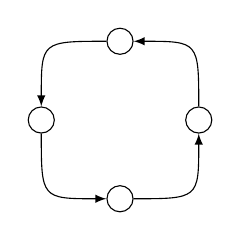
\begin{tikzpicture}
      \tikzstyle{every node}=[circle]
      \node[draw] (n1) at (1,0) {};
      \node[draw] (n2) at (2,1) {};
      \node[draw] (n3) at (1,2) {};
      \node[draw] (n4) at (0,1) {};
    	
      \draw[-latex] (n3) .. controls +(-1,0) .. (n4) {};
      \draw[-latex] (n4) .. controls +(0,-1) .. (n1) {};
      \draw[-latex] (n1) .. controls +(1,0) .. (n2) {};
      \draw[-latex] (n2) .. controls +(0,1) .. (n3) {};
    \end{tikzpicture}\end{tabular} & \begin{tabular}[c]{l} \texttt{x:Node --> .\ --> .\ --> .\ --> x;} \end{tabular}\\
  & \\  
  \begin{tabular}[c]{c}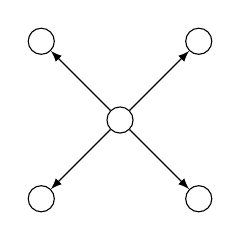
\begin{tikzpicture}
      \tikzstyle{every node}=[circle]
      \node[draw] (n1) at (1,1) {};
      \node[draw] (n2) at (0,0) {};
      \node[draw] (n3) at (0,2) {};
      \node[draw] (n4) at (2,0) {};
      \node[draw] (n5) at (2,2) {};
    	
      \draw[-latex] (n1) -- (n2) {};
      \draw[-latex] (n1) -- (n3) {};
      \draw[-latex] (n1) -- (n4) {};
      \draw[-latex] (n1) -- (n5) {};
    \end{tikzpicture}\end{tabular} & \begin{tabular}[c]{l} \texttt{.\ <-- x:Node --> .;} \\ \texttt{.\ <-- x --> .;} \end{tabular}\\
  & \\
  \begin{tabular}[c]{c}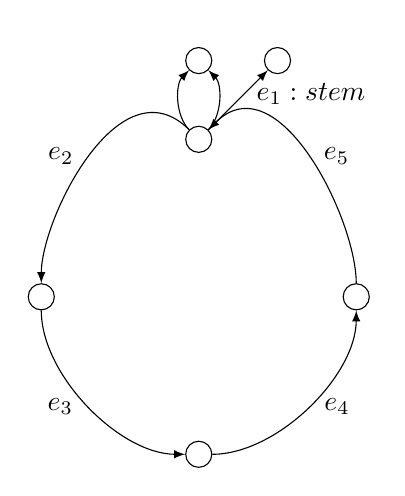
\begin{tikzpicture}
      \tikzstyle{every node}=[circle]
      \node[draw] (n1) at (3,5) {};
      \node[draw] (n2) at (2,4)   {};
      \node[draw] (n3) at (0,2)   {};
      \node[draw] (n4) at (2,0)   {};
      \node[draw] (n5) at (4,2)   {};
      \node[draw] (n6) at (2,5.0)   {};
    	
    	\draw[-latex] (n2) --                                  (n1) node[right,pos=0.6] {$e_1:\text{stem}$};
    	\draw[-latex] (n2) .. controls +(-1,1) and +(0,1) ..   (n3) node[left,midway]  {$e_2$};
      \draw[-latex] (n3) .. controls +(0,-1) and +(-1,0) ..  (n4) node[left,midway]  {$e_3$};
    	\draw[-latex] (n4) .. controls +(1,0)  and +(0,-1) ..  (n5) node[right,midway] {$e_4$};
      \draw[-latex] (n5) .. controls +(0,1)  and +(1,1) ..   (n2) node[right,midway] {$e_5$};
    	\draw[-latex] (n2) .. controls +(-0.3,+0.3) and +(-0.3,-0.3) .. (n6) node[left,midway]   {};
    	\draw[-latex] (n2) .. controls +(+0.3,+0.3) and +(+0.3,-0.3) .. (n6) node[right,midway]  {};
    \end{tikzpicture}\end{tabular} & \begin{tabular}[c]{l} \texttt{.\ <-e1:stem- n1:Node -e2:Edge-> .\ -e3:Edge-> .} \\ \quad\texttt{-e4:Edge-> .\ -e5:Edge-> n1;}\\ \texttt{n1 --> n2:Node;} \\ \texttt{n1 --> n2;} \end{tabular}\\
   & \\
  \begin{tabular}[c]{c}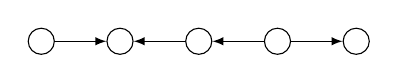
\begin{tikzpicture}
      \tikzstyle{every node}=[circle]
      \node[draw] (n1) at (0,0) {};
      \node[draw] (n2) at (1,0) {};
      \node[draw] (n3) at (2,0) {};
      \node[draw] (n4) at (3,0) {};
      \node[draw] (n5) at (4,0) {};
    	
      \draw[-latex] (n1) -- (n2) {};
      \draw[-latex] (n3) -- (n2) {};
      \draw[-latex] (n4) -- (n3) {};
      \draw[-latex] (n4) -- (n5) {};
    \end{tikzpicture}\end{tabular} & \begin{tabular}[c]{l} \texttt{.\ --> .\ <-- .\ <-- .\ --> .;} \end{tabular} \\
  & \\
  \begin{tabular}[c]{c}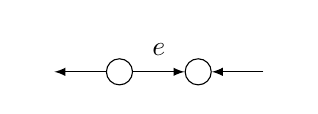
\begin{tikzpicture}
      \tikzstyle{every node}=[circle]
      \node (n1) at (0,0) {};
      \node[draw] (n2) at (1,0) {};
      \node[draw] (n3) at (2,0) {};
      \node (n4) at (3,0) {};
    	
      \draw[-latex] (n2) -- (n1) {};
      \draw[-latex] (n2) -- (n3) node[midway,above] {$e$};
      \draw[-latex] (n4) -- (n3) {};
    \end{tikzpicture}\end{tabular} & \begin{tabular}[c]{l} \texttt{-e:Edge->} \\ \texttt{<-- .\ -e-> .\ <--\ ;} \end{tabular}
\end{tabular}\\
\end{center}
\mbox{ }\\
\mbox{ }\\
\mbox{ }\\
And some illegal graphlets:\\
\mbox{}\\
\mbox{}\\
\begin{tabularx}{\linewidth}{cX}
\texttt{.\ -e:Edge-> .; .\ -e-> .;} & Would affect redirecting of edge \texttt{e}. \\
 & \\
 \texttt{x -e:T-> y; x -e-> x;} & Would affect redirecting of edge \texttt{e}. \\
  & \\
 \texttt{x:Node; negative \{y:Node; hom(x,y)\}} & Here \texttt{x} must not occur in the \texttt{hom} statement. See Section~\ref{patternpart} for further information. \\
  & \\
  \texttt{<-- --> ;} & There must be at least a node between the edges.
\end{tabularx}
\end{example}
\end{figure}

\begin{note}
Although both, the pattern part and the replace/modify part use graphlets, there are subtle differences between them. These concern the \emph{TypeConstraint} clause, the retype operator \texttt{<>}, and the scope of defined graph element names: Names defined within the pattern part are valid in the pattern part as well as in the replace/modify part. Names defined within the replace/modify part are unknown to the pattern part.
\end{note}

\section{Rules and Tests}
\label{ruledecls}
The structure of a \indexed{rule set} file is as follows:
\begin{rail}
  RuleSet: 'actions' IdentDecl (() | 'using' ((ModelIdent)+',')) ';' \\ ((TestDeclaration | RuleDeclaration)+) ;
\end{rail}\ixkeyw{actions}\ixkeyw{using}\ixnterm{RuleSet}
A rule set consists of the underlying \indexed{graph model}s and several rewrite rules. In case of multiple graph models, \GrG\ uses the union of these models. In this case beware of conflicting declarations. There is no built-in conflict resolution mechanism like packages or namespaces for models. If necessary you can use prefixes as you might do in C.

\begin{rail}
  TestDeclaration: 'test' ActionSignature lbrace Pattern rbrace ;
  RuleDeclaration: 'rule' ActionSignature lbrace Pattern Replace rbrace ;
\end{rail}\ixkeyw{test}\ixkeyw{rule}\ixnterm{TestDeclaration}\ixnterm{RuleDeclaration}
Declares a single \indexed{rewrite rule} such as \texttt{SomeRule}. It consists of a pattern part (see Section~\ref{patternpart}) in conjunction with its rewrite/modify part (see Section~\ref{replacepart}). A \newterm{test} has no rewrite specification. It's intended to check whether (and maybe how many times) a pattern occurs.
\begin{example}
We define a test \texttt{SomeCond}
\begin{grgen}
test SomeCond {
  pattern {
    n: SeldomNodeType;
  }
}
\end{grgen}
and execute in \GrShell:
\begin{grshell}
  grs SomeCond & SomeRule
\end{grshell}
SomeRule will only be executed, if a node of type \texttt{SeldomNodeType} exists. For graph rewrite sequences in \GrShell\ see Section~\ref{grsthings}.
\end{example}

\begin{rail}  
  ActionSignature: IdentDecl (() | Parameters) (() | ':' ReturnTypes) ;
\end{rail}\ixnterm{ActionSignature}
The \indexed{signature} sets the name of a rewrite rule to \emph{IdentDecl} and optionally names and types of formal \indexed{parameter}s as well as a list of \indexed{return type}s. Parameters and return types provide users with the ability to exchange graph elements with rule. This is similar to parameters of procedural languages.

\begin{rail}
  Parameters: '(' ((IdentDecl ':' NodeType | '-' IdentDecl ':' EdgeType '->') + ',') ')' ;
\end{rail}\ixnterm{Parameters}
Within a rule, parameters are treated as (predefined) graph elements of the pattern. Even if a supplied parameter value is undefined\indexmain{undefined parameter}, it is treated as valid node or edge definition. So in any case a graph element of the specified type has to be mapped. \GrG\ assumes the lookup operation for parameters to be in $\mathcal{O}(1)$. In case of an undefined parameter value this might lead to bad \indexed{search plan}s, because \GrG\ has to actually search for such a graph element.
\begin{figure}[htbp]
\begin{example}
Assume the following \indexed{test} that checks whether the edge \texttt{e} is not \indexed{incident} to \texttt{x}:
\begin{grgen}
test r(-e:Edge->, x:Node) {
  pattern {
    negative {
      -e-> x;
    }
    negative {
      x <-e-;
    }
  }
}
\end{grgen}
If \texttt{x} and \texttt{e} are undefined, test \texttt{r} is equivalent to test \texttt{s}:
\begin{grgen}
test s {
  pattern {
    x:Node;
    -e:Edge->;
    negative {
      -e-> x;
    }
    negative {
      x <-e-;
    }
  }
}
\end{grgen}
In particular, test \texttt{s} is successful if there is \emph{some} edge in the host graph that is \emph{not} incident to \texttt{x}.
\end{example}
\end{figure}

\begin{rail}
  ReturnTypes: '(' ((NodeType | EdgeType) + ',') ')' ;
\end{rail}\ixnterm{ReturnTypes}
The return types specify edge and node types of graph elements that are returned by the replace/modify part. If return types are specified, the \texttt{return} statement is mandatory. Otherwise no \texttt{return} statement must occur. See also Section~\ref{replacepart}, \texttt{return}.
\begin{figure}[htbp]
\begin{example}\label{ex:rule:someruleext}
We extend \texttt{SomeRule} (Example~\ref{ex:rule:SomeRule}) with a user defined node to match and we want it to return the rewritten graph elements \texttt{n5} and \texttt{e1}.
\begin{grgen}
  rule SomeRuleExt(varnode: Node): (Node, EdgeTypeB) {
    pattern {
      n1: NodeTypeA;
      ...
    }
    replace {
      varnode;
      ...  
      return(n5, e1);
      eval {
        ...
\end{grgen}
We don not define \texttt{varnode} within the pattern part because this is already covered by the parameter specification itself.
\end{example}
\end{figure}

\section{Pattern Part}\indexmain{pattern}
\label{patternpart}
\begin{rail}
  Pattern: 'pattern' lbrace (()+PatternStatement) rbrace ;
\end{rail}\ixkeyw{pattern}\ixnterm{Pattern}
A \indexed{pattern} consists of zero or more pattern statements. 
All the pattern statements must be fulfilled by a subgraph of the host graph in order to form a match. 
An \indexed{empty pattern} always produces exactly one (empty) match. 
This is caused by the uniqueness of the total and totally undefined function.

Names defined for graph elements may be used by other pattern statements as well as by replace/modify statements. 
Like all identifier definitions, such names may be used before their \indexed{declaration}. 
See Section~\ref{rulebb} for a detailed explanation of names and graphlets.
\begin{figure}[htbp]
\begin{note}
\label{note:indeterminism}
The \indexed{application} of a rule is not deterministic\indexmain{non-determinism}\indexmainsee{determinism}{non-determinism} (remember the example of the introduction in Section~\ref{ov:example}); in particular there may be more than one subgraph that matches the pattern. 
Whereas the \GrShell\ selects one of them arbitrarily (without further abilities to control the selection), the underlying \LibGr\indexmain{libGr} provides a mechanism to deal with such ambiguities. 
\LibGr\ allows for splitting a rule application into two steps: Find all the subgraphs of the host graph that match the pattern and rewrite one of these matches. 
By returning a collection of all matches, the \LibGr\ retains the complete graph rewrite process under control.
As a \LibGr\ user use the following methods of the \texttt{IAction} interface:
\begin{csharplet}
IMatches Match(IGraph graph, int maxMatches, IGraphElement[] parameters);
IGraphElement[] Modify(IGraph graph, IMatch match);
\end{csharplet}
In C\#, this might look like:
\begin{csharplet}
IMatches myMatches = myAction.Match(myGraph, -1, null); /* -1: get all the matches */
for (int i = 0;  i < myMatches.NumMatches; i++)
{
	if (inspectCarefully(myMatches.GetMatch(i))
	{
		myAction.Modify(myGraph, myMatches.GetMatch(i));
		break;
  	}
}
\end{csharplet}

Also notice that \indexed{graph rewrite sequence}s introduce a further variant of non-determinism on rule application level: 
The \indexed{\texttt{\$<op>}} flag marks the operator \texttt{<op>} as commutative, i.e.\ the execution order of its operands (rules) is non-deterministic. 
See Section~\ref{grsthings} for further information on graph rewrite sequences.
\end{note}
\end{figure}

\begin{rail}  
  PatternStatement: 
    Graphlet ';' |
    'hom' '(' (Ident + ',') ')' ';' |
    'negative' lbrace (()+PatternStatement) rbrace |
    'if' lbrace (BooleanExpr ';' +) rbrace |
    'return' '(' (Ident+',') ')' ';' ;
\end{rail}\ixkeyw{hom}\ixkeyw{negative}\ixkeyw{if}\ixkeyw{return}\ixnterm{PatternStatement}
The semantics of the various pattern statements are given below:
\begin{description}
  \item[Graphlet] \indexmain{graphlet}Graphlets specify connected subgraphs. See Section~\ref{rulebb} for a detailed explanation of graphlets. 
  \item[Isomorphic/Homomorphic Matching] \indexmain{isomorphic matching}\indexmain{homomorphic matching}The \texttt{hom} operator specifies the nodes or edges that may be matched homomorphically. 
  In contrast to the default isomorphic matching, the specified graph elements \emph{may} be mapped to the same graph element in the host graph. Note that the graph elements must have a common subtype. 
  Several homomorphically matched graph elements will be mapped to a graph element of a common subtype.
  In Example~\ref{ex:rule:SomeRule} nodes \texttt{n1} and \texttt{n2} may be the same node. This is possible because they are of the same type (\texttt{NodeTypeA}).
  A name may not occur in multiple \texttt{hom} statements. 
  For instance it is illegal to write \texttt{hom(a, b); hom(b, c);}. Instead write \texttt{hom(a, b, c);}. 
  Inside a NAC the \texttt{hom} operator may only operate on graph elements that are either defined or used in the NAC.
  \item[Negative Application Conditions (NACs)] \indexmain{negative application condition}\indexmainsee{NAC}{negative application condition}With negative application conditions (keyword \texttt{negative}) we can specify graph patterns which forbid the application of a rule if any of them is present in the host graph (cf.~\cite{adam}). 
  NACs must not be nested.
  NACs possess a \indexed{scope} of their own. 
  Names defined within a NAC do not exist outside the NAC. 
  Identifiers from surrounding scopes must not be redefined.
  In general NACs do not care about bindings within the outer scope. 
  Nevertheless, if you use an identifier that is defined in the outer scope, this specifies exactly the graph element, the identifier is bound to in the outer scope.
  \begin{example}
    We specify a node \texttt{x} with out-degree of exactly 2:
    \begin{grgen}
pattern {
  <-- x:Node -->;
  negative {
    <-- x -->;
    x -->;
  }
}
    \end{grgen}
  \end{example}
  \item[Attribute Conditions] \indexmain{attribute condition}The Java-like attribute conditions (keyword \texttt{if}) in the pattern part allow for further restriction of the applicability of a rule.
  \item[Return values] \indexmain{return value}The return statement is only allowed for tests. Otherwise the \texttt{return} statement belongs to the replace part. See Section~\ref{replacepart}, \emph{Return Values}.
\end{description}
Keep in mind that using type constraints or the \texttt{typeof} operator can be helpful. See Section~\ref{typeexpressions} for further information.

\section{Replace/Modify Part}\indexmain{replacement graph}
\label{replacepart}
For the task of rewriting, \GrG\ provides two different modes: A \emph{replace mode} and a \emph{modify mode}.

\subsection{Implicit Definition of the Preservation Morphism\indexmain{preservation morphism} $r$}
\label{rule:morphismr}
Besides specifying the pattern, a main task of a rule is to specify the transformation of a matched subgraph within the \indexed{host graph}. 
The \indexed{transformation specification} defines the transition from the \indexed{left hand side} (LHS) to the \indexed{right hand side} (RHS), i.e.\ which graph elements of a match will be kept, which of them will be deleted and which graph elements have to be newly created.
In theory this is done by defining the preservation morphism $r$.
\begin{figure}[htbp]
	\centering
  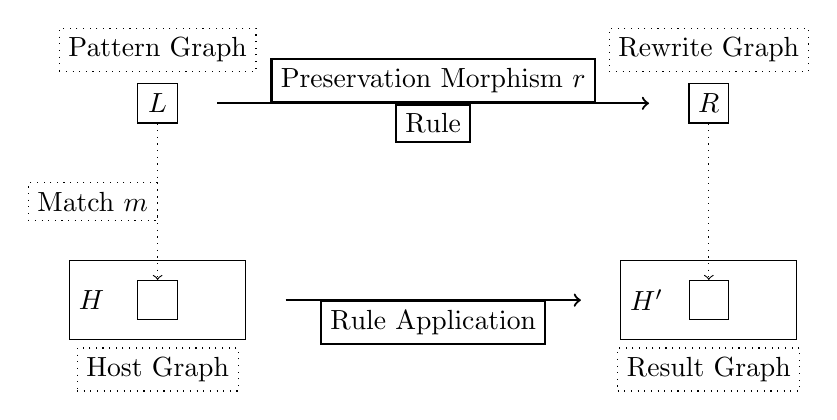
\begin{tikzpicture}
    \begin{scope}[minimum size=0.5cm]
      \tikzstyle{every node}=[draw]
      \node (L)     at (0   ,2.5) {$L$};
      \node (R)     at (7   ,2.5) {$R$};
      \node (mL)    at (0   ,0) {};
      \node (mR)    at (7   ,0) {};
      \node[text width=2cm,text badly ragged,minimum size=1cm] (H)     at (0   ,0) {$H$};
      \node[text width=2cm,text badly ragged,minimum size=1cm] (Hs)    at (7   ,0) {$H'$};
    \end{scope}

    \draw[dotted,->] (L) node[above=0.4cm] {Pattern Graph} -> (mL) node[left,midway]  {Match $m$}   node[below=0.6cm] {Host Graph};
    \draw[dotted,->] (R) node[above=0.4cm] {Rewrite Graph} -> (mR)                              node[below=0.6cm] {Result Graph};

    \pgfsetshortenstart{0.5cm}
    \pgfsetshortenend{0.5cm}
    \draw[thick,->]  (L) -> (R)  node[above,midway] {Preservation Morphism $r$} node[below,midway] {Rule};
    \draw[thick,->]  (H) -> (Hs) node[below,midway] {Rule Application};
  \end{tikzpicture}
  \caption{Process of Graph Transformation}
  \label{rule:figrule}
\end{figure}
In \GrG\, the preservation morphism $r$ is defined implicitly by using \indexed{name}s both in pattern \indexed{graphlet}s and replace graphlets (we don not need to care about the the differences of the replace part and the modify part at the moment).
Remember that to each of the graph elements a name is bound to, either user defined or internally defined. If such a name is used in a replace graphlet, the denoted graph element will be kept. 
Otherwise the graph element will be deleted.
By defining a name in a replace graphlet a corresponding graph element will be newly created.
So in a replace pattern \indexed{anonymous} graph elements will always be created.
Using a name multiple times has the same effect as a single using occurrence.
In case of a conflict between \indexed{deletion} and \indexed{preservation}, deletion is prioritized. 
If an incident node of an edge gets deleted, the edge will be deleted as well (in compliance to the SPO\indexmain{single-pushout approach} semantics).

\begin{table}[htbp]
\centering
\begin{tabularx}{\linewidth}{lllX}
  \textbf{Pattern (LHS)} & \textbf{Replace (RHS)} & \textbf{$r: L \longrightarrow R$} & \textbf{Meaning} \\ \hline 
  \texttt{x:T;} & \texttt{x;}                 & $r:\lhs.x \mapsto \rhs.x$ & Preservation \\
  \texttt{x:T;} & \texttt{}                   & $\lhs.x \notin \deF(r)$    & Deletion \\
  \texttt{} & \texttt{x:T;}                   & $\rhs.x \notin \ran(r)$    & Creation \\
  \texttt{x:T;} & \texttt{x:T;}               & --- & Illegal, redefinition of \texttt{x} \\
  \texttt{-e:T->;} & \texttt{-e-> x:Node;}    & --- & Illegal, redirection of  \texttt{e} \\
  \texttt{x:N -e:E-> y:N;} & \texttt{x -e->;} & $r:\{\lhs.x\} \mapsto \{\rhs.x\}$ & Deletion of \texttt{y}. Hence del\-etion of \texttt{e}. \\
\end{tabularx}
\caption{Definition of the preservation morphism $r$}
\label{rule:impldefinition}
\end{table}



\subsection{Specification Modes for Graph Transformation}

\begin{description}
  \item[Replace mode] \indexmain{replace mode}The semantics of this mode is to delete every graph element of the pattern that is not used (occur) in the replace part, keep every graph element that is used, and create every additionally defined graph elements. ``Using'' means that the name of a graph element occurs in a graphlet. Attribute calculations are no using occurrences.\\
  In Example~\ref{ex:rule:someruleext} the nodes \texttt{varnode} and \texttt{n3} will be kept. The node \texttt{n1} is replaced by the node \texttt{n5} preserving \texttt{n1}'s edges. The anonymous edge instance between \texttt{n1} and \texttt{n2} only occurs in the pattern and therefore gets deleted.\\
See Section~\ref{rule:morphismr} for a detailed explanation of the transformation semantics. 
  \item[Modify mode] The \indexed{modify mode} can be regarded as a replace part in replace mode, where every pattern graph element is added (occurs) before the first replace statement. 
In particular all the \indexed{anonymous} graph elements are kept. 
Additionally this mode supports the \texttt{delete} operator that deletes every element given as an argument. 
Deletion takes place after all other rewrite operations. Multiple deletion of the same graph element is allowed (but pointless) as well as deletion of just created elements (pointless, too).
\begin{figure}[htbp]
\begin{example}
How might Example~\ref{ex:rule:someruleext} look in modify mode? 
We have to denominate the anonymous edge between \texttt{n1} and \texttt{n2} in order to delete it. 
The node \texttt{varnode} should be kept and does not need to appear in the modify part. 
So we have
\begin{grgen}
rule SomeRuleExtModify(varnode: Node): (Node, EdgeTypeB)  {
  pattern {
    ...
    n1 -e0:Edge-> n2;
    ...
  }
  modify {
    n5 : NodeTypeC<n1>;
    n3 -e1:EdgeTypeB-> n5;
    delete(e0);
    eval {
      ...
\end{grgen}
\end{example}
\end{figure}
\end{description}

\subsection{Syntax}

\begin{rail}
  Replace: ('replace' | 'modify') lbrace (()+ReplaceStatement) rbrace ;
\end{rail}\ixkeyw{replace}\ixkeyw{modify}\ixnterm{Replace}
Selects whether the replace mode or the modify mode is used. Several replace statements describe the transformation from the pattern subgraph to the destination subgraph.

\begin{rail}  
  ReplaceStatement: Graphlet ';' |
    'delete' '(' (Ident + ',') ')' ';' |
    'eval' lbrace (Assignment ';' +) rbrace |
    'return' '(' (Ident+',') ')' ';' ;
\end{rail}\ixkeyw{delete}\ixkeyw{eval}\ixkeyw{return}\ixnterm{ReplaceStatement}
The semantics of the various pattern statements are given below:
\begin{description}
  \item[Graphlet] \indexmain{graphlet}Analogous to a pattern graphlet; a specification of a connected subgraph. Its graph elements are either kept because they are elements of the pattern or added otherwise. Names defined in the pattern part must not be redefined in the replace graphlet. See Section~\ref{rulebb} for a detailed explanation of graphlets. 
  \item[Deletion] \indexmain{deletion}The \texttt{delete} operator is only available in the modify mode. It deletes the specified pattern graph elements. Multiple occurrences of \texttt{delete} statements are allowed. Deletion statements are executed after all other replace statements. Multiple deletion of the same graph element is allowed (but pointless) as well as deletion of just created elements (pointless, too).
  \item[Attribute Evaluation] \indexmain{attribute evaluation}\indexmainsee{evaluation}{attribute evaluation}\indexmainsee{re-evaluation}{attribute evaluation}If a rule is applied, then the attributes of matched and inserted graph elements will be recalculated according to the \texttt{eval} statements.
  \item[Return Values] \indexmain{return value}Graph elements of the replace/modify part can be returned according to the return types in the signature (see Section~\ref{ruledecls}, \texttt{ActionSignature}). The \texttt{return} statement must not occur multiple times. The graph element names have to be in the same order as the corresponding return types in the signature. The named elements must be compatible to the declared type.
  \item[Retyping] \indexmain{retyping}Retyping enables us to keep all adjacent nodes and all attributes stemming from common super types of a graph element while changing its type (table~\ref{rule:retyping_graphlets} shows how retyping can be expressed both for nodes and edges).
  Retyping differs from a \indexedsee{type cast}{retyping}: During replacement both of the graph elements are alive.
  Specifically both of them are available for evaluation, a respective evaluation could, e.g., look like this:
  \begin{grgenlet}
eval {
  y.b = (2*x.i == 42 );
  f.a = e.a;
}
  \end{grgenlet}
  Furthermore the source and destination types need \emph{not} to be on a path in the directed \indexed{type hierarchy} graph, rather their relation can be arbitrary.
  However, if source and destination type have one ore more common super types, then the respective attribute values are adopted by the retyped version of the respective node (or edge).
  The edge specification as well as \emph{ReplaceNode} supports retyping. 
  In Example~\ref{ex:rule:SomeRule} node \texttt{n5} is a retyped node stemming from node \texttt{n1}.
  Note, that---conceptually---the retyping is performed \emph{after} the SPO conform rewrite.
\end{description} 

\begin{table}[htbp]
\centering
\begin{tabularx}{\linewidth}{lllX}
  \textbf{Pattern (LHS)} & \textbf{Replace (RHS)} & \textbf{$r: L \longrightarrow R$} & \textbf{Meaning} \\ \hline 
  \texttt{x:N1;} & \texttt{y:N2<x>;}          & $r:\lhs.x \mapsto \rhs.x$ & Preserve \texttt{x}, then retype \texttt{x} from \texttt{N1} to \texttt{N2} and bind name \texttt{y} to retyped version of \texttt{x}.\\
  \texttt{e:E1;} & \texttt{f:E2<e>;}          & $r:\lhs.e \mapsto \rhs.e$ & Preserve \texttt{e}, then retype \texttt{e} from \texttt{E1} to \texttt{E2} and bind name \texttt{f} to the retyped version of \texttt{e}.\\
\end{tabularx}
\caption{Retyping of preserved nodes and edges}
\label{rule:retyping_graphlets}
\end{table}










\begin{rail}    
   Assignment: Ident '.' Ident '=' Expression ;
\end{rail}\indexmain{attribute evaluation}\ixnterm{Assignment}
Several evaluation parts are allowed within the replace part. Multiple evaluation statements will be internally concatenated, preserving their order. Evaluation statements have \indexedsee{imperative}{attribute evaluation} semantics. In particular, \GrG\ does not care about data dependencies. Evaluation takes place before any graph element gets deleted and after all the new elements have been created. You may read (and write, although this is pointless) attributes of graph elements to be deleted.
\begin{example}
\begin{grgen}
...
modify {
  ...
  eval {y.i = 40;}
  eval {y.j = 0;}
  x: IJNode;
  y: IJNode;
  delete(x);
  eval {
    x.i = 1; 
    y.j = x.i;
    x.i = x.i + 1;
    y.i = y.i + x.i;
  }
\end{grgen}
This toy example yields $\texttt{y.i} = 42$, $\texttt{y.j} = 1$.
\end{example}


